\chapter{Design}
\label{chap:design}

This chapter explains the design process undertaken considering both the research found within the literature review \see{chap:litrev} and the established requirements \see{chap:requirements}.
\section{Assumptions and Decisions Taken}
\label{design:assumptions/decisions}

Discussions with the client required specific assumptions and decisions to be made to assit in the project's overall development and progression.

A decision was made to build the application as a web app, primarily to aid with accessibility and device compatibility of the artefact, this type of application also opens the artefact up to a large pre-existing userbase with greater ease. Different screen sizes have been acommodated for with the use of CSS media queries, however the artefact is aimed at desktop route planning, with the potential to be expanded to support mobile devices in the future. 

It was assumed that the target users would have a preexisting knolwedge of route planning and had used similar systems in the past. Due to this, instructions to use the application were not provided as a part of the artefact. Futhermore, a minimal user interface approach was used when developing the artefact to ensure the apps ease of use, whilst enabling key custom route planning functionality \see{design:ui}.

Research was undertaken into different available open source routing algorithms, finally deciding to implement Open Route Service (\cite{noauthor_openrouteservice_nodate}) due to its customisability and native support of round trip route planning.

Specific data sets were stored within the browser LocalStorage, this was chosen for certain data such as user authentication tokens, last route plotted and other data which needed storing between browser sessions. Data sets such as the previous planned route (and related data sets) enabled the user to load the previous route when opening the application after having closed the tab/browser previously. Other data sets such as user tokens, enabled the application to remain logged into external services such as Strava (\cite{noauthor_strava_nodate}), Garmin Connect (\cite{international_garmin_nodate}) and Google Drive (\cite{noauthor_home_nodate}), only requiring the user to reauthenticate once these tokens had expired.

\section{User Interface}
\label{design:ui}
Initially, multiple hand-drawn low-fidelity protoype was created to demonstrate two iterations of the artefact \see{fig:lofi1}, demonstrating some design changes and new features in the second low-fidelity prototype \see{fig:lofi2}. After the low-fidelity prototypes were complete, a high fidelity prototype was created based on the second design using MarvelApp (\cite{noauthor_marvel_nodate}).

The following 5 components form the overall User Interface (UI): Map,  Elevation Chart, Router, Route Preferences Panel and the Weather/Side Panel. The primary component which most other components were dependant on was the Map component; each other component would add enhanced functionality to the artefact.

\subsection{Colour Scheme}
\label{ui:colourscheme}

The plain and simple colour scheme was chosen for simplicity and ease-of-use of the artefact. Despite dark mode being considered for the artefact, it was chosen against after conducting research on pre-existing route planners, it was found that a light map, and surrounding UI was generally considered more usable to the average user. A dark mode could be implemented in the future, enabling the user to switch modes should they choose, also altering the map layer to the corresponding dark/light theme.

\subsection{Low Fidelity Prototype}
\label{ui:low-fi}

Low-fidelity protoyping was vital in the project's early stages, ensuring that all UI elements would meet the user expectations and requirements. The project's clear focus on enhanced routing features, it was critical to ensure that the initialy designs were kept simple, to maximise usability, whilst still including all the required, key functionality. Two iterations were divided into two separate low-fidelity prototypes, where the first demonstrates the core functionality \see{fig:lofi1}, whereas the second also includes some extra functionality, for example the Hazard Index \see{fig:lofi2}.

\subsection{High-Fidelity Prototype}
\label{ui:hi-fi}

The high-fidelity prototype was made after low-fidelity prototyping has concluded. The second low-fidelity prototype was expanded upon at this stage, keeping the design simple, whilst ensuring the required functionality could be implemented. It was critical to ensure tthe high-fidelity protype wouldn't overbare the user with too much information at once, therefore the necessary functionality is available in the main view \see{fig:hifi1}, whereas extra options are hidden behind dropdown menus \see{fig:hifi2}.

  \begin{figure}[!ht]
    \centering
    \includegraphics[width=350px]{figures/lofi-1.png}
    \caption{Low-Fidelity Prototype 1}
    \label{fig:lofi1}
  \end{figure}

  \begin{figure}[!ht]
    \centering
    \includegraphics[width=350px]{figures/lofi-2.png}
    \caption{Low-Fidelity Prototype 2}
    \label{fig:lofi2}
  \end{figure}

  \begin{figure}[!ht]
    \centering
    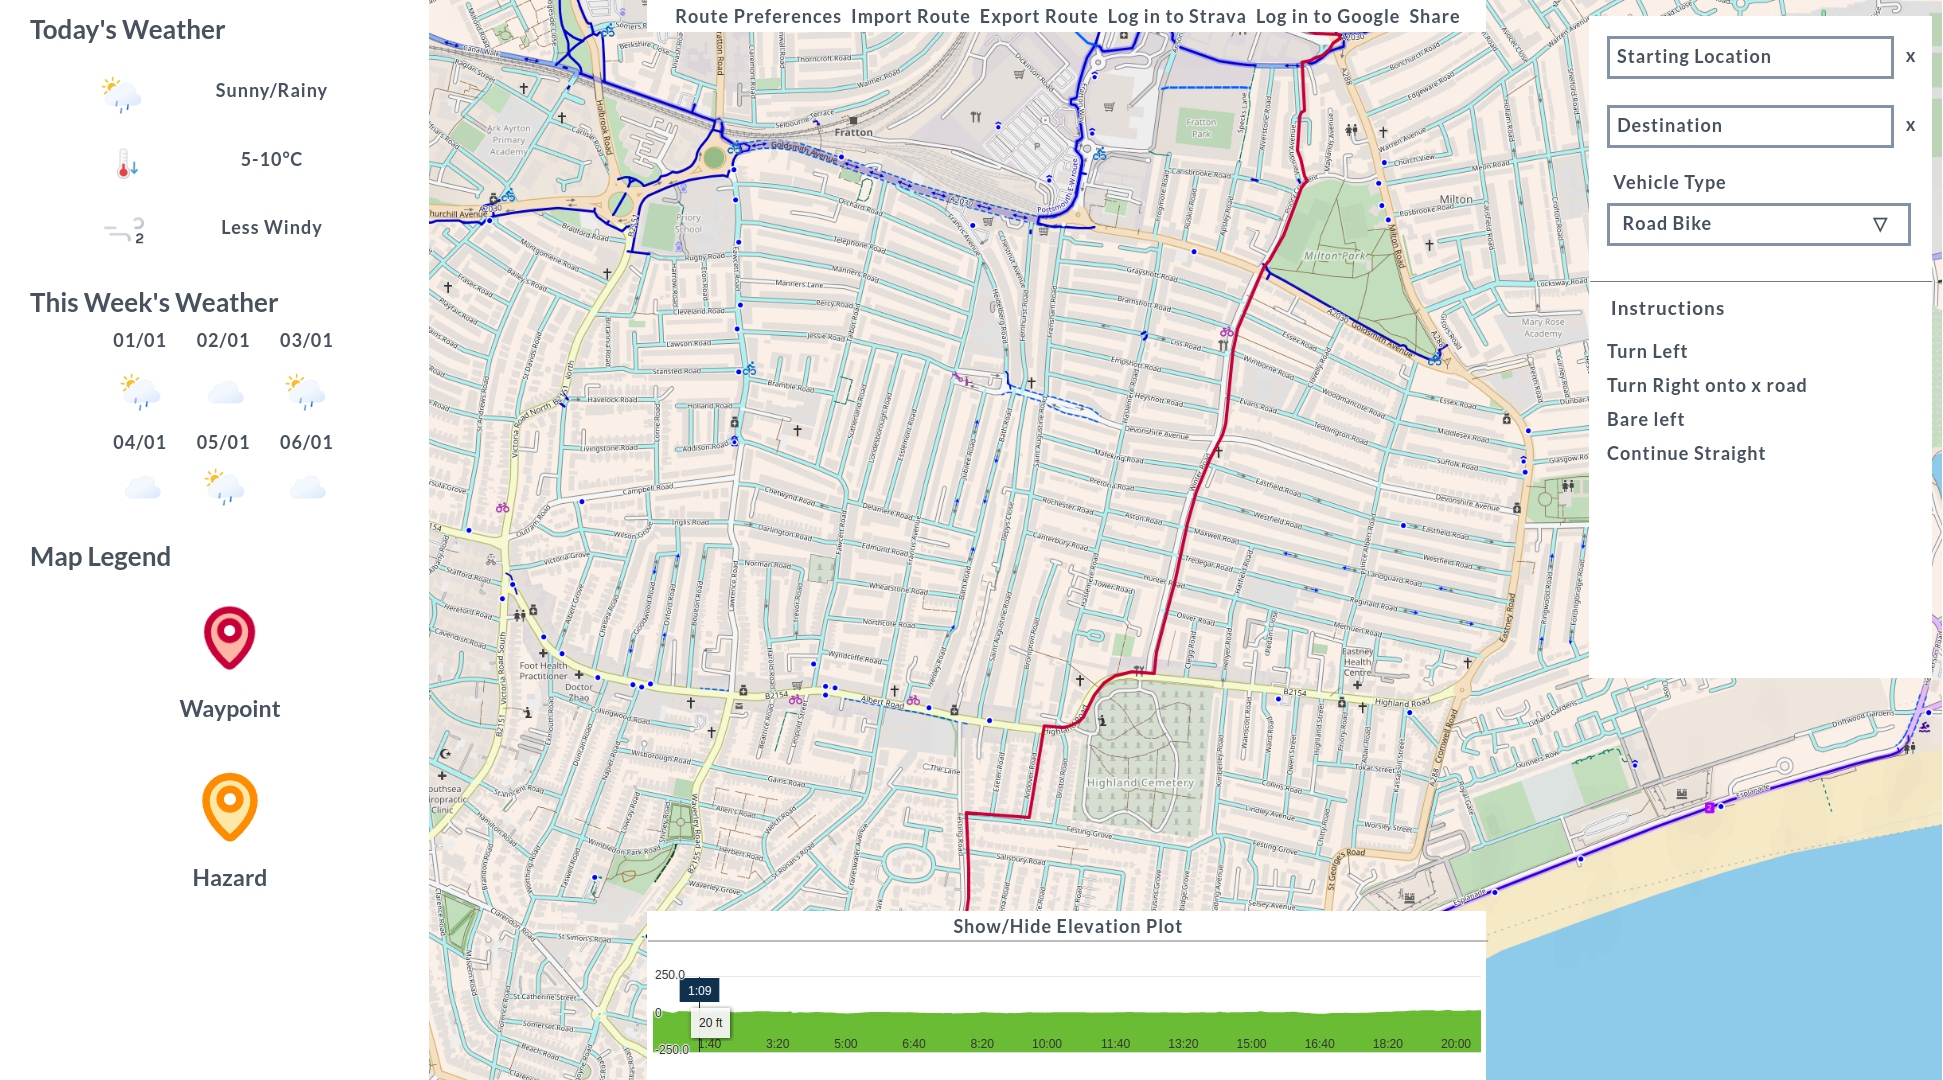
\includegraphics[width=400px]{figures/hifi-1.png}
    \caption{High-Fidelity Prototype 1}
    \label{fig:hifi1}
  \end{figure}

  \begin{figure}[!ht]
    \centering
    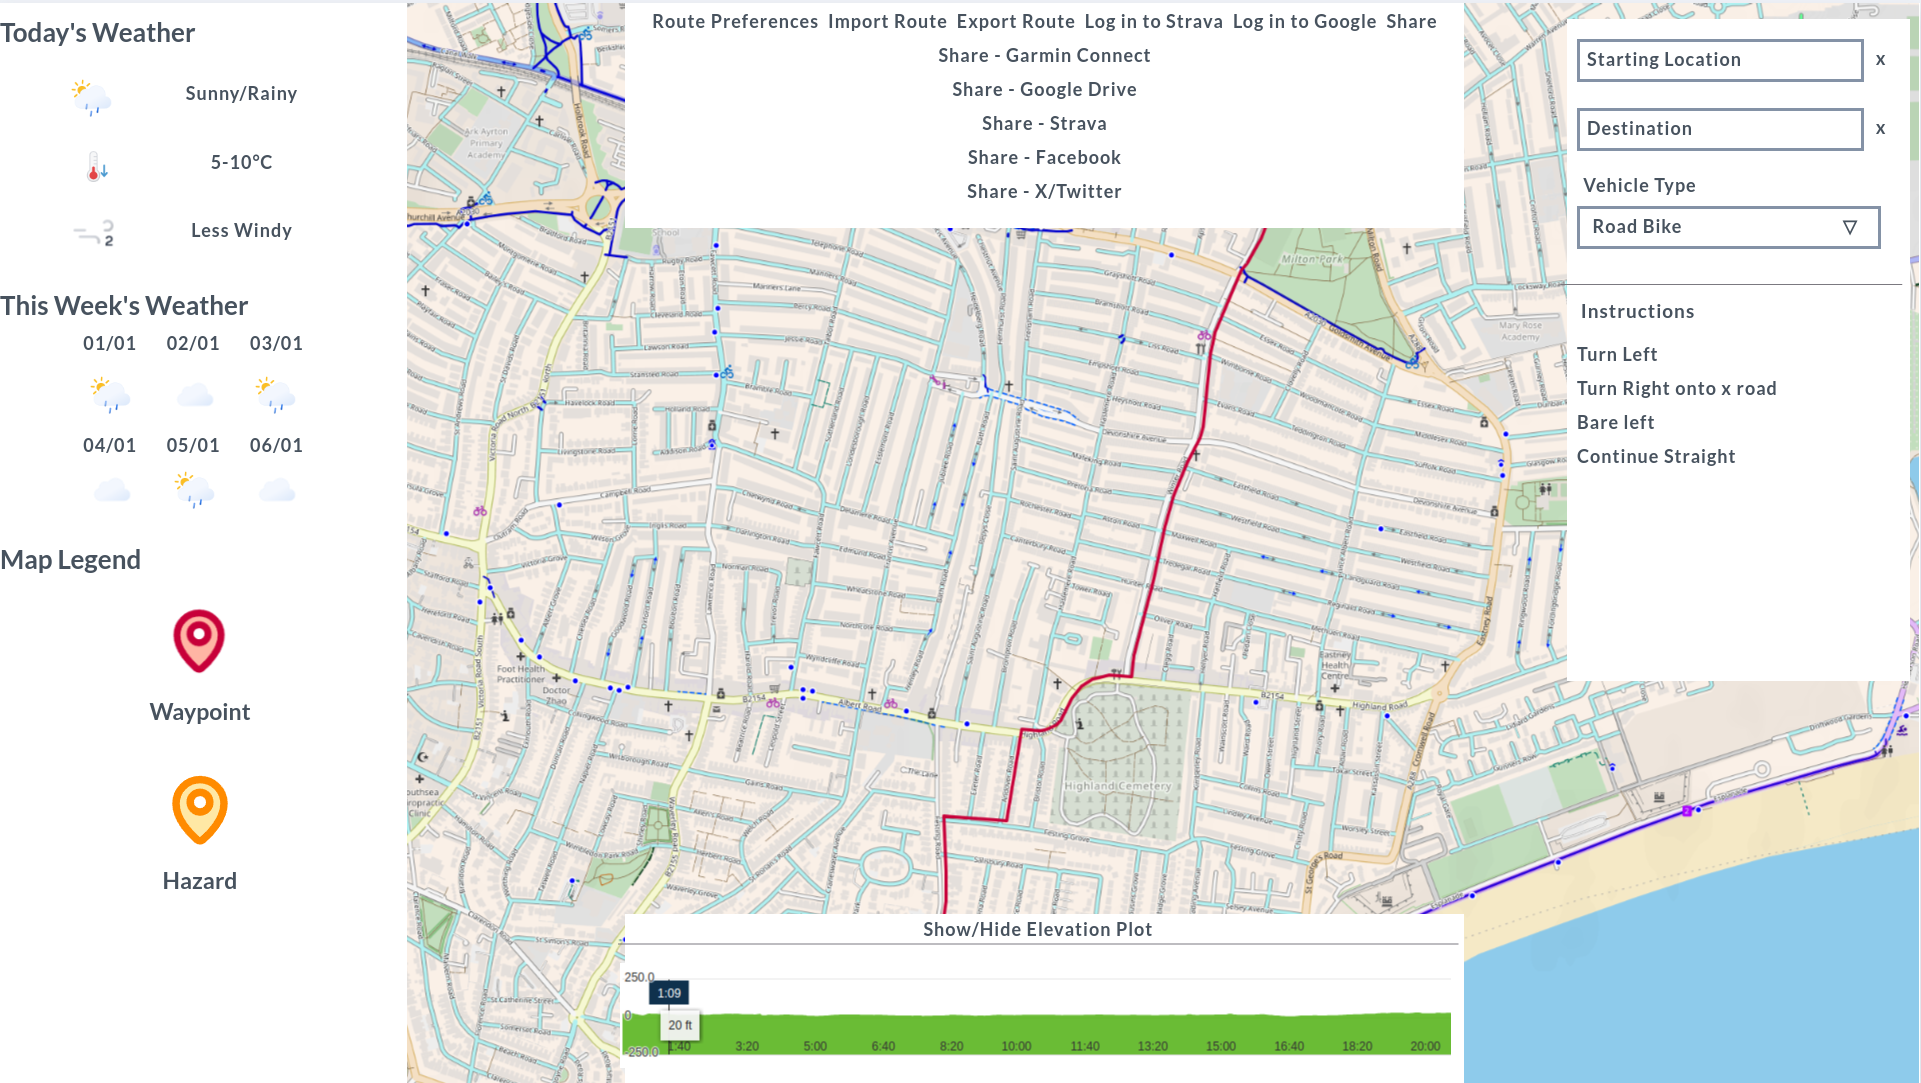
\includegraphics[width=400px]{figures/hifi-2.png}
    \caption{High-Fidelity Prototype 2}
    \label{fig:hifi2}
  \end{figure}

  \clearpage
\section{Use Cases}
\label{design:usecase}
Use cases were determined by discerning potential uses of the artefact, subsequently a use case diagram was then created to visualise the artefacts different uses. The diagram is formed of actors, tasks and system components which are requred to response when each task is performed. Visual Paradigm was used to create the use case diagram (\cite{noauthor_ideal_nodate}).

\subsection{Use Case Diagram}
\label{usecase:diagram}
During the requirements gathering process, the target user groups were identified, each user group would access identical functionality \see{chap:requirements}, therefore all users were grouped into one single actor. Doing so enables all users to access all functionalities of the artefact, where they can use as little or as many of the extended features as they require \see{fig:usecase}.

\begin{figure}[!ht]
  \centering
  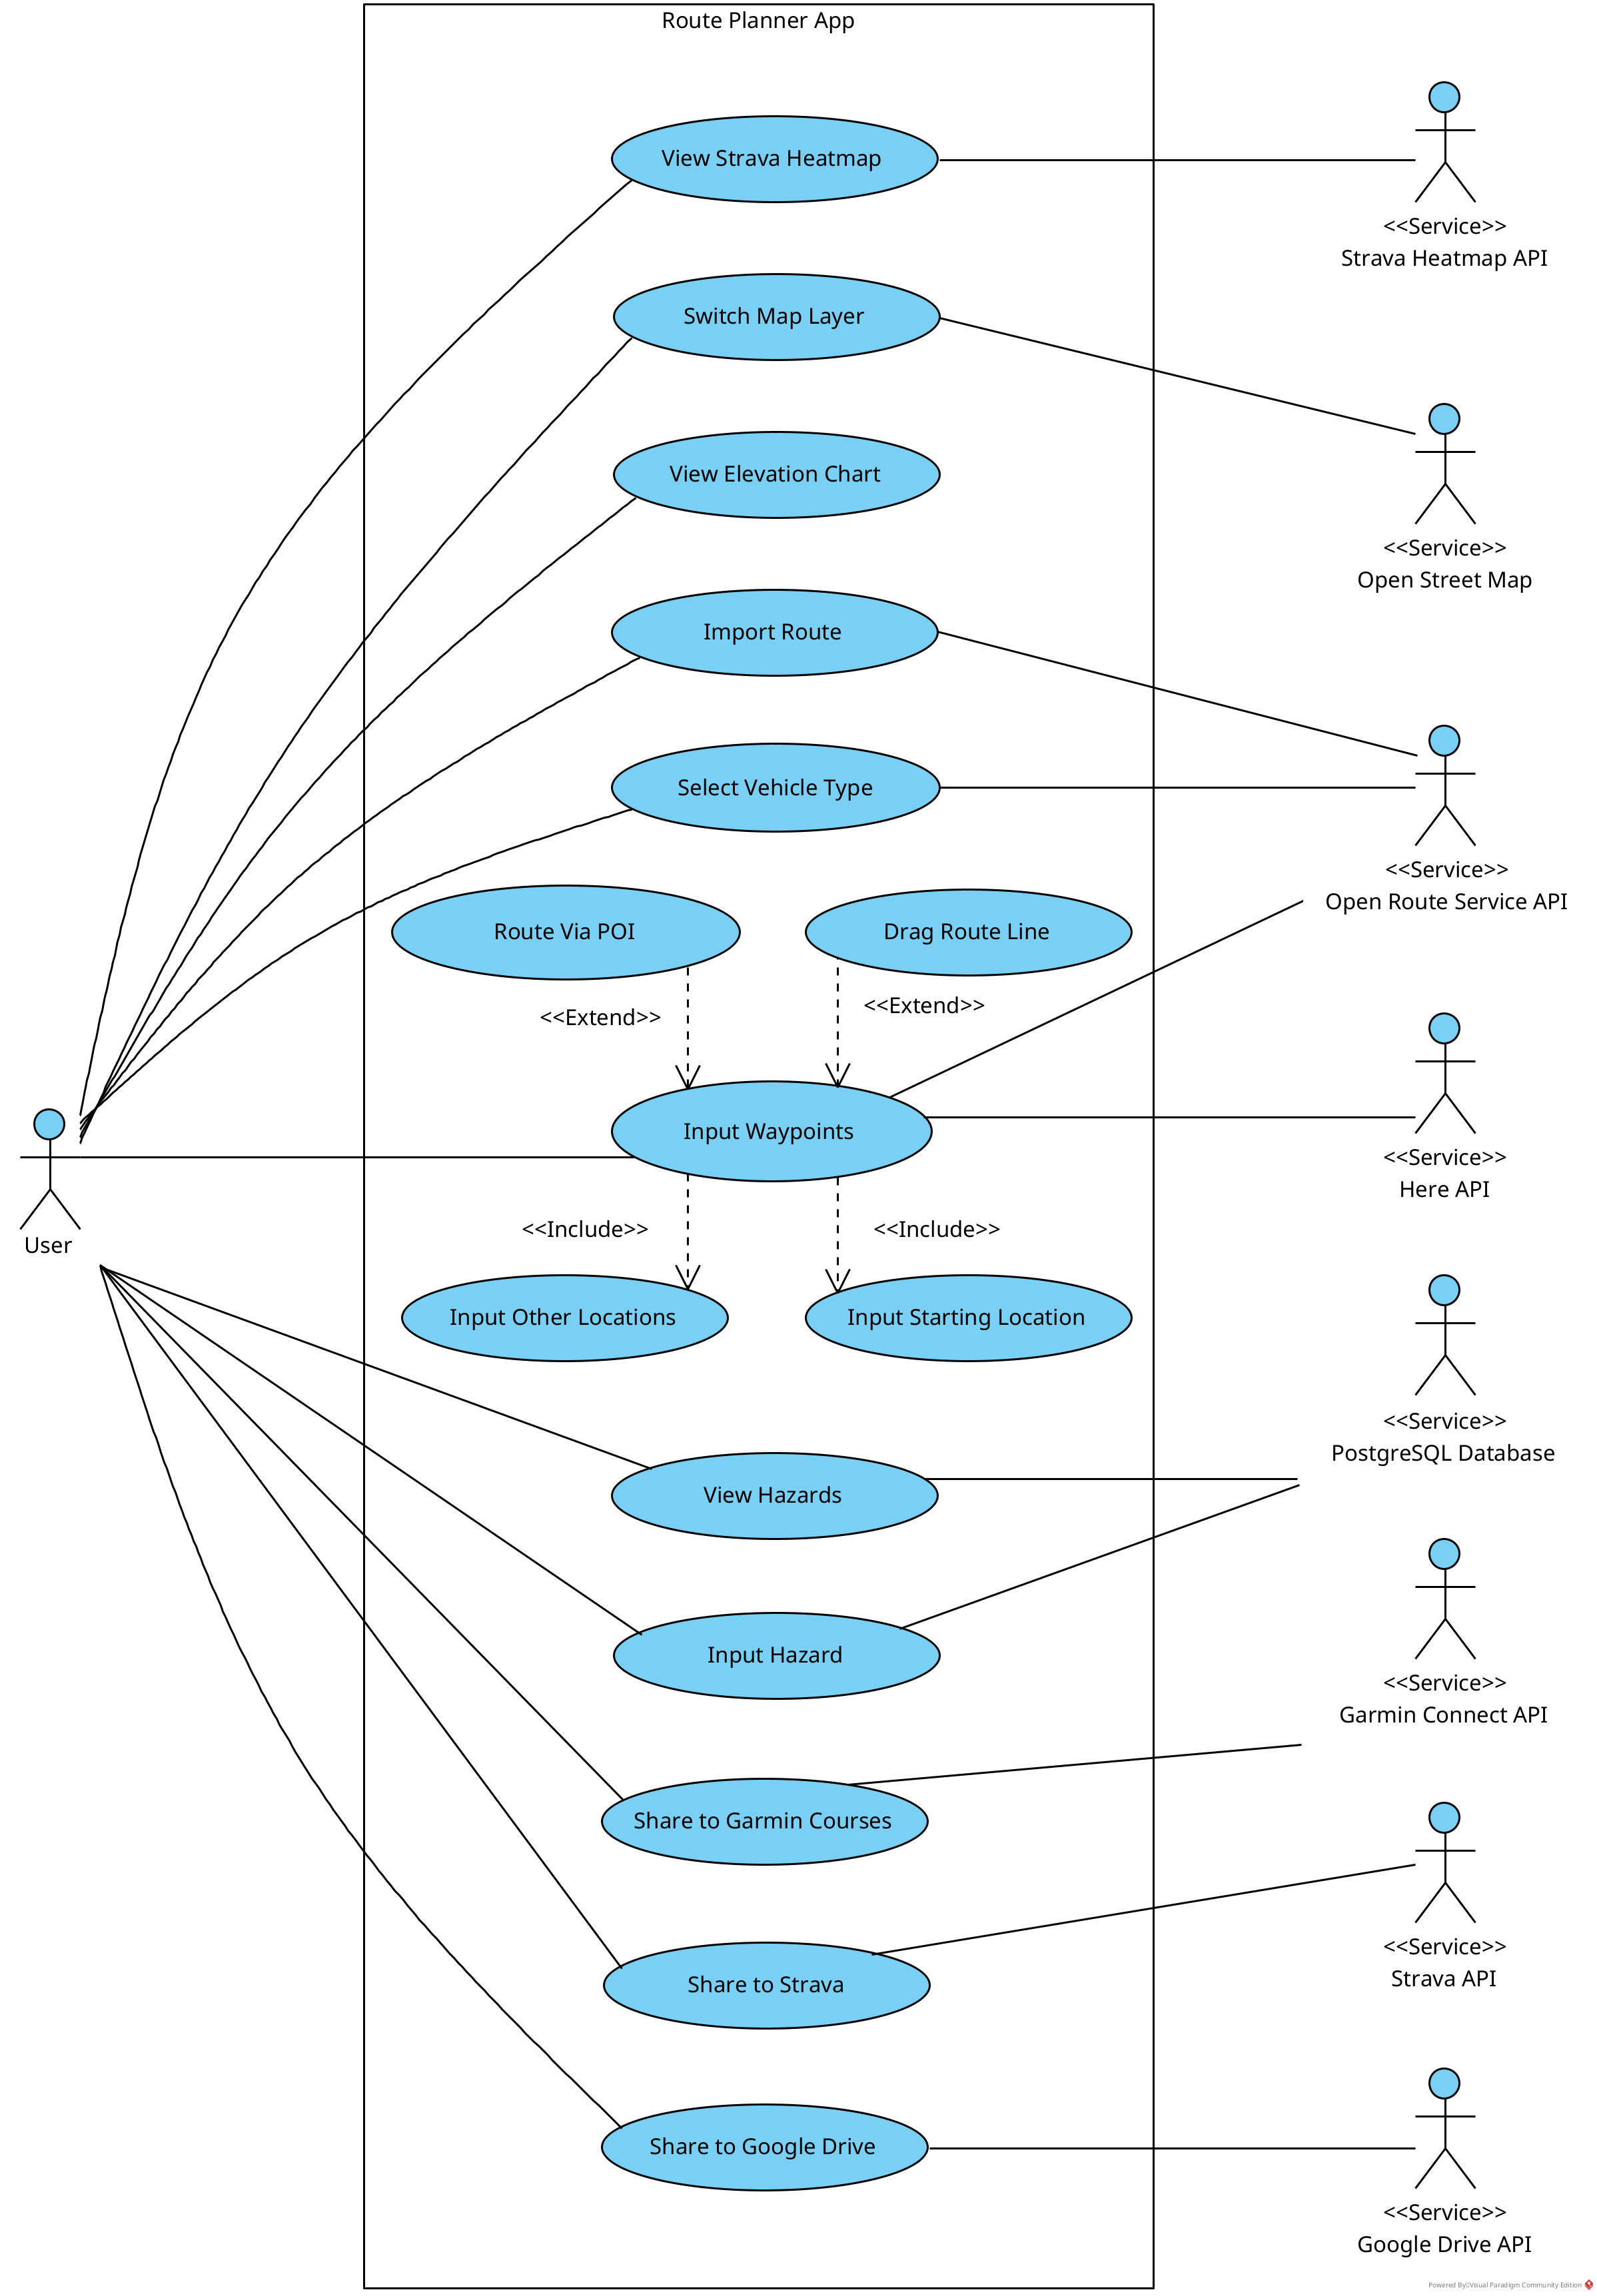
\includegraphics[width=400px]{figures/use-case.png}
  \caption{Use Case Diagram}
  \label{fig:usecase}
\end{figure}

\section{System Design}
\label{design:system}

It is vital to design not only the viewable client-side of the application, but to also consider the internal system, comprising of the Go Gin Web Server, PostgreSQL database as well as the React.js client. This chapter delves further into the internal design of the artefact. 

\subsection{Architecture Design}
\label{system:architecture-design}

The client-server architecture was used to build the artefact \see{fig:clientserver}. This architecture was selected to enable easy expansion of the artefact, with the aim for the web application to be hosted centrally, along with the PostgreSQL (PSQL) database \see{system:database-design}. For security reasons, it was also necessary to implement this architecture due to different services requiring oauth, these services make enforce authentication through the server, rather than completely on the client-side application. Furthermore, this architecture enabled different processes to be handled via the server, reducing the overall load the client application requires to run.

Client-Server architectures do however, add the risk of a single point of failure, whereby the application is wholly dependant on the web server. Overall the risk was deemed minimal due to the lack of sensitive information being stored \see{tab:risk-assessment}. In the case of a system failure, the application would remain unaccessable until fixed, however there is a low chance of this occurring as the appropriate measures such as thorough testing have been undertaken to reduce the risk \see{chap:testing}.

\clearpage
\begin{figure}[!ht]
  \centering
  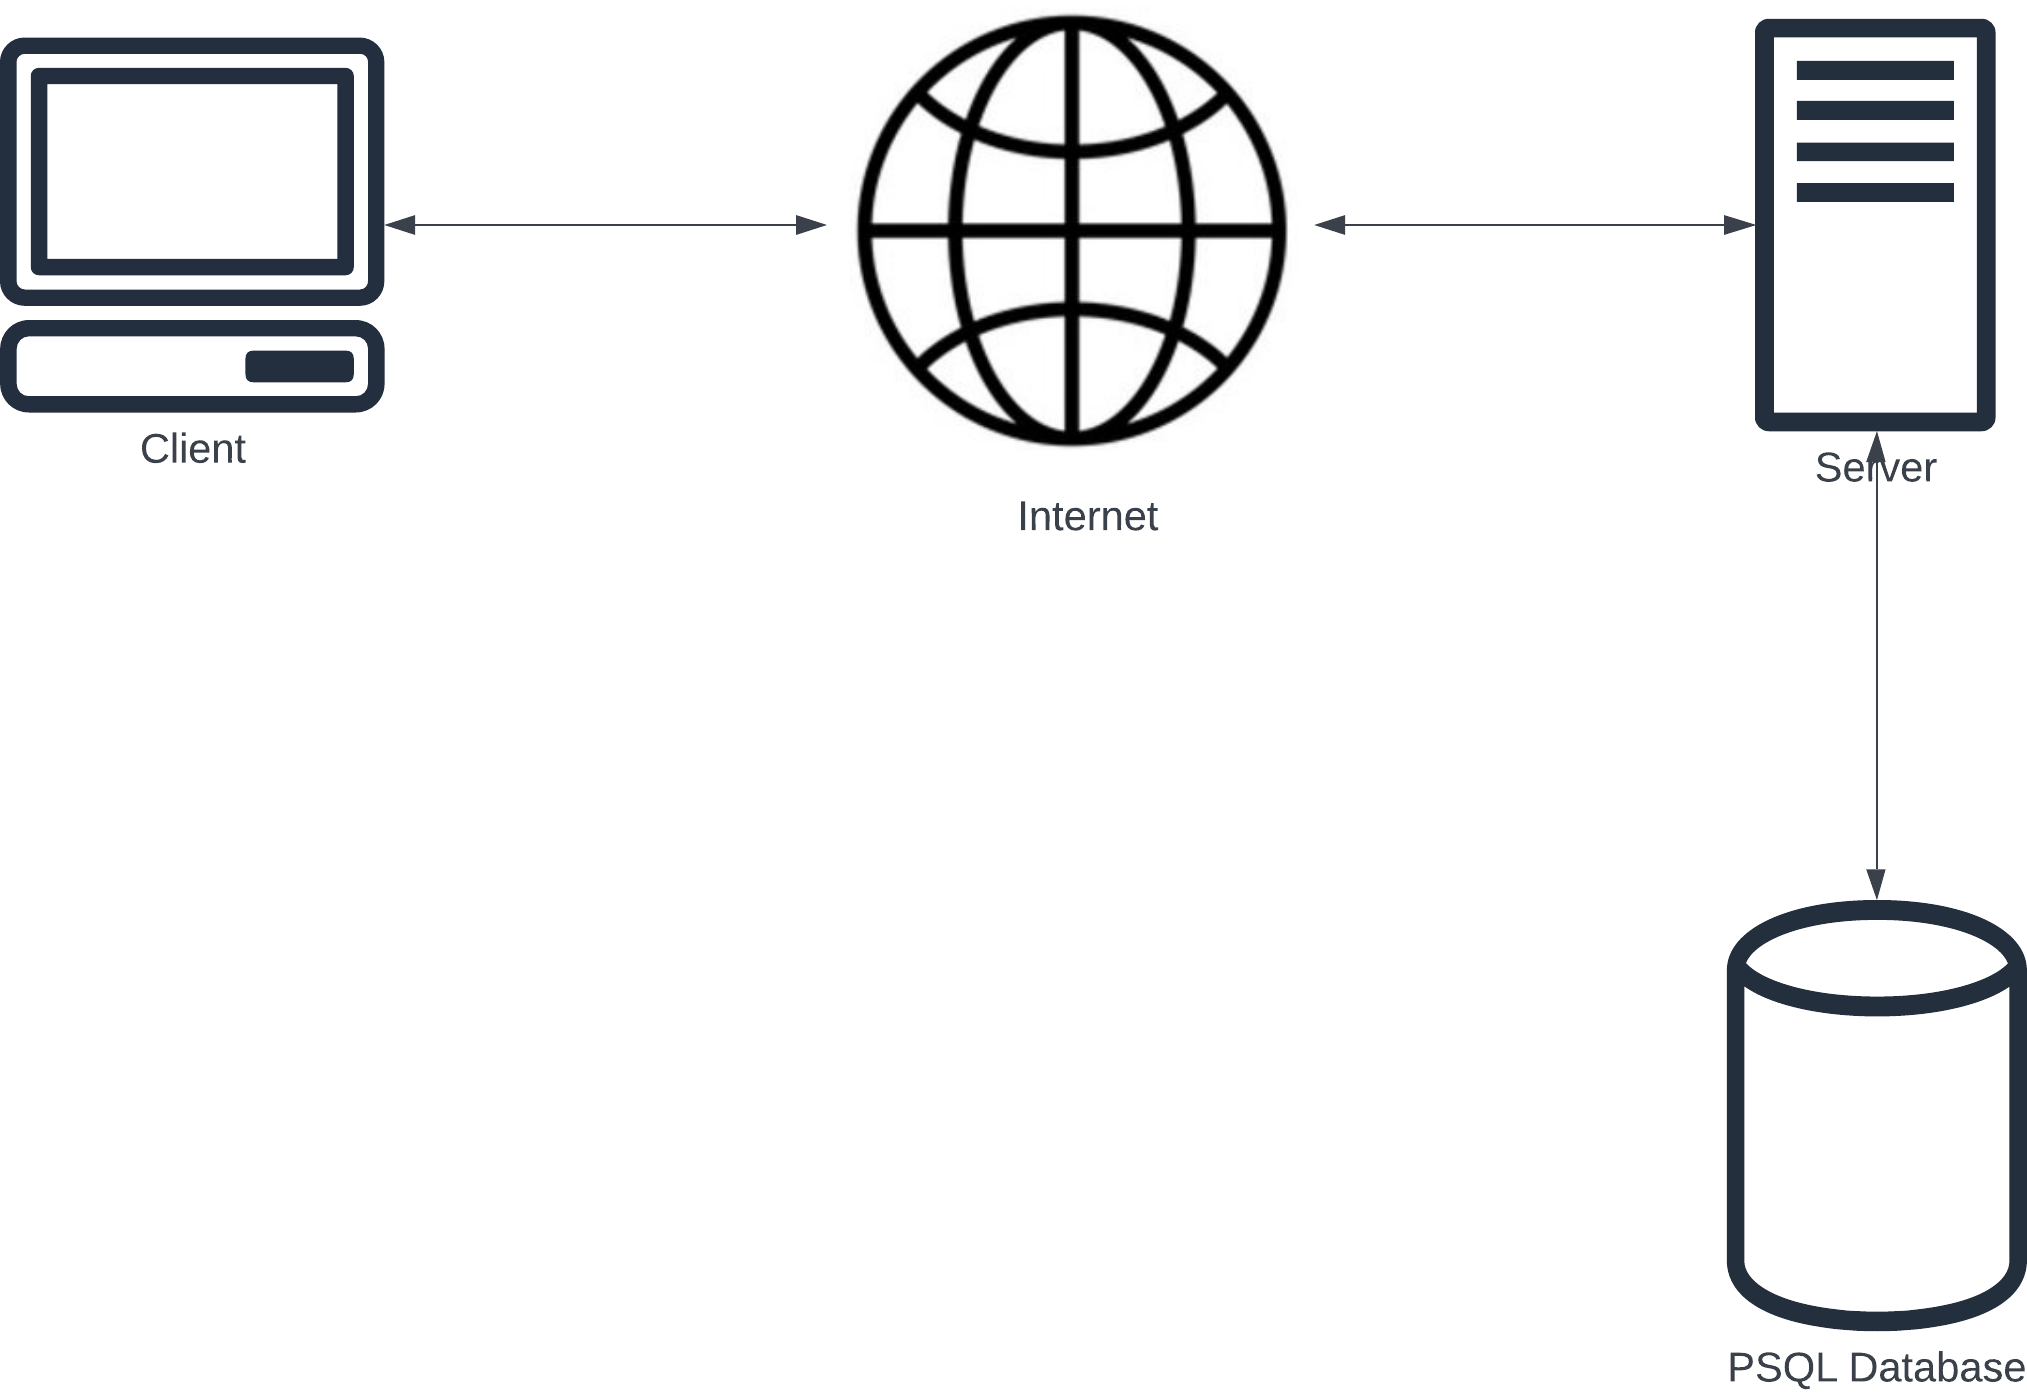
\includegraphics[width=250px]{figures/client-server.png}
  \caption{Client-Server Architecture}
  \label{fig:clientserver}
\end{figure}

\subsection{Database Design}
\label{system:database-design}

The database is a pivitol part of the artefact's extended functionality, it primarily servers as a hazard index database, whilst also storing different areas of concerning cycling infrastructure. PostgreSQL was chosen as the Relational Database Management System (RDBMS), as PostGIS was available to use to add the functionality for storing, indexing and querying of geospacial data (\cite{noauthor_postgis_nodate}). This data is used to display concerning areas on the map for which users may want to avoid, with the potential to include native routing support to avoid these hazards, futher highlighted under future work \see{evaluation:future} \see{fig:erd}. 

\begin{figure}[!ht]
  \centering
  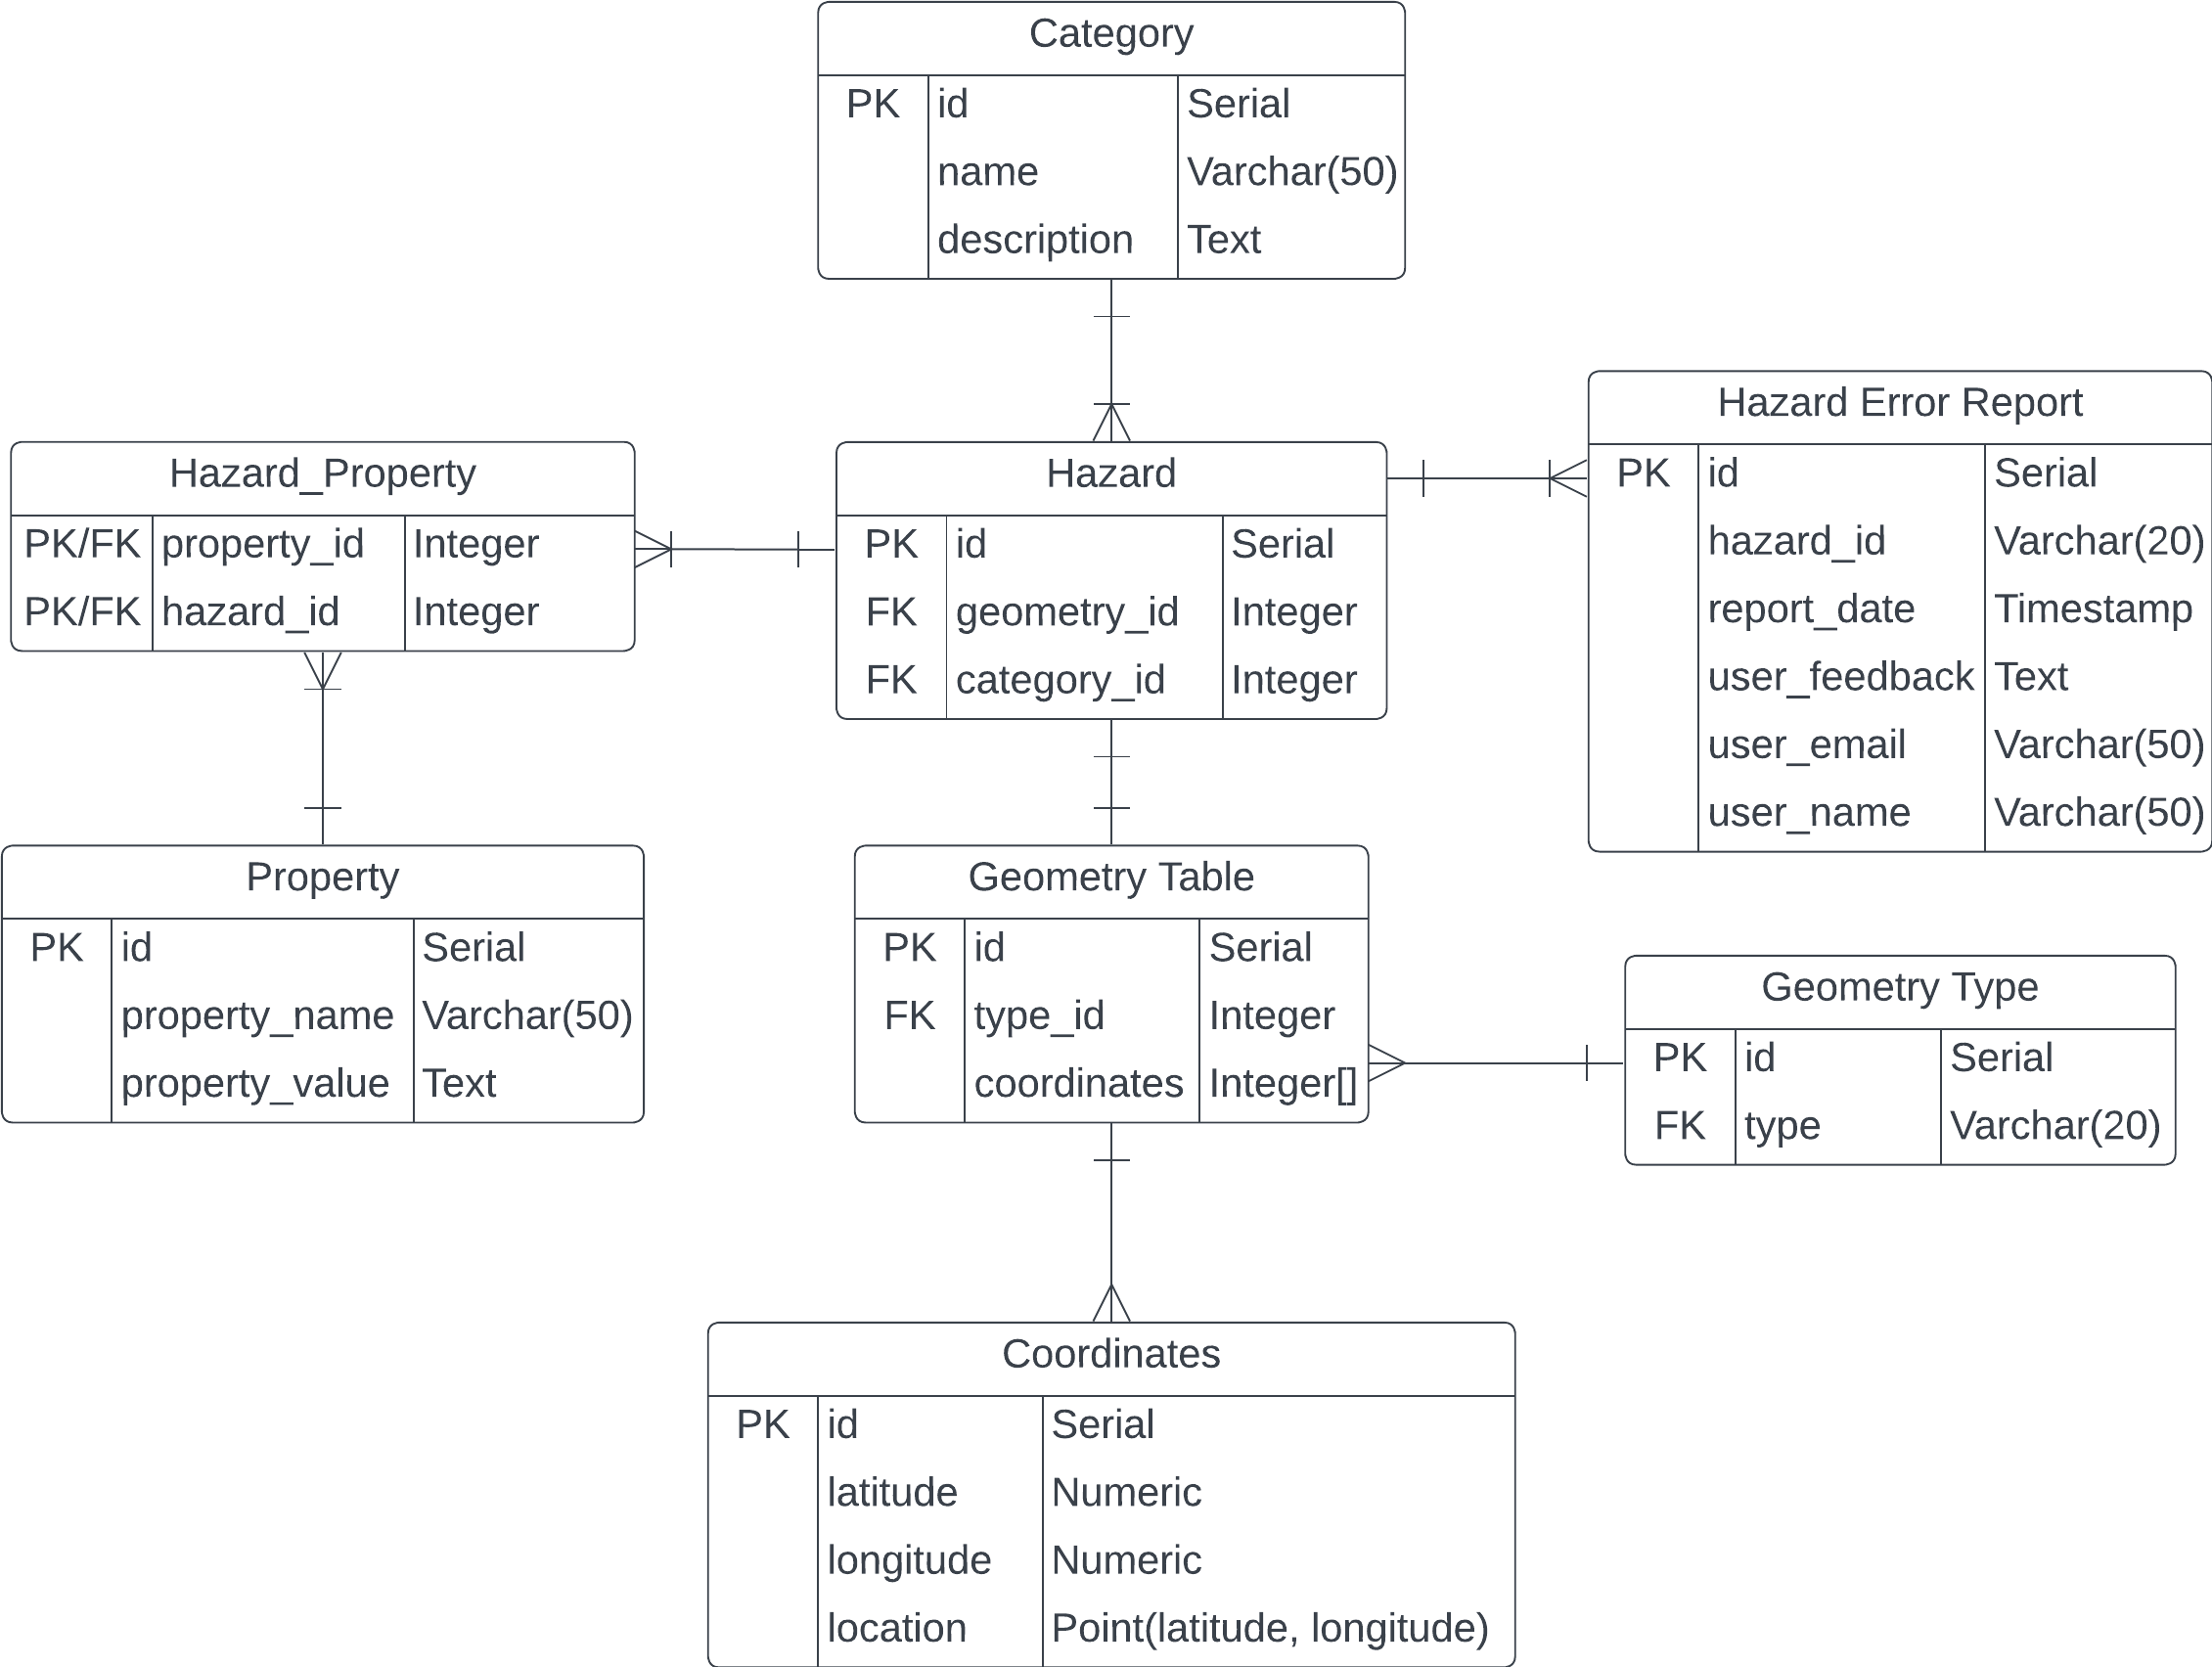
\includegraphics[width=350px]{figures/erd.png}
  \caption{Entity Relationship Diagram}
  \label{fig:erd}
\end{figure}

\subsection{Module Architecture}
\label{system:module-architecture}
React.js allows for a modular design approach utilising the component-based framework and storing variables in the form of states to re-render the application dependant on the states of different variables. All the necessary data, functions and states can be passed to and from different components using the props functionality built into React, whereby a component inherits data from its parent component \see{fig:components}.  

\begin{figure}[!ht]
  \centering
  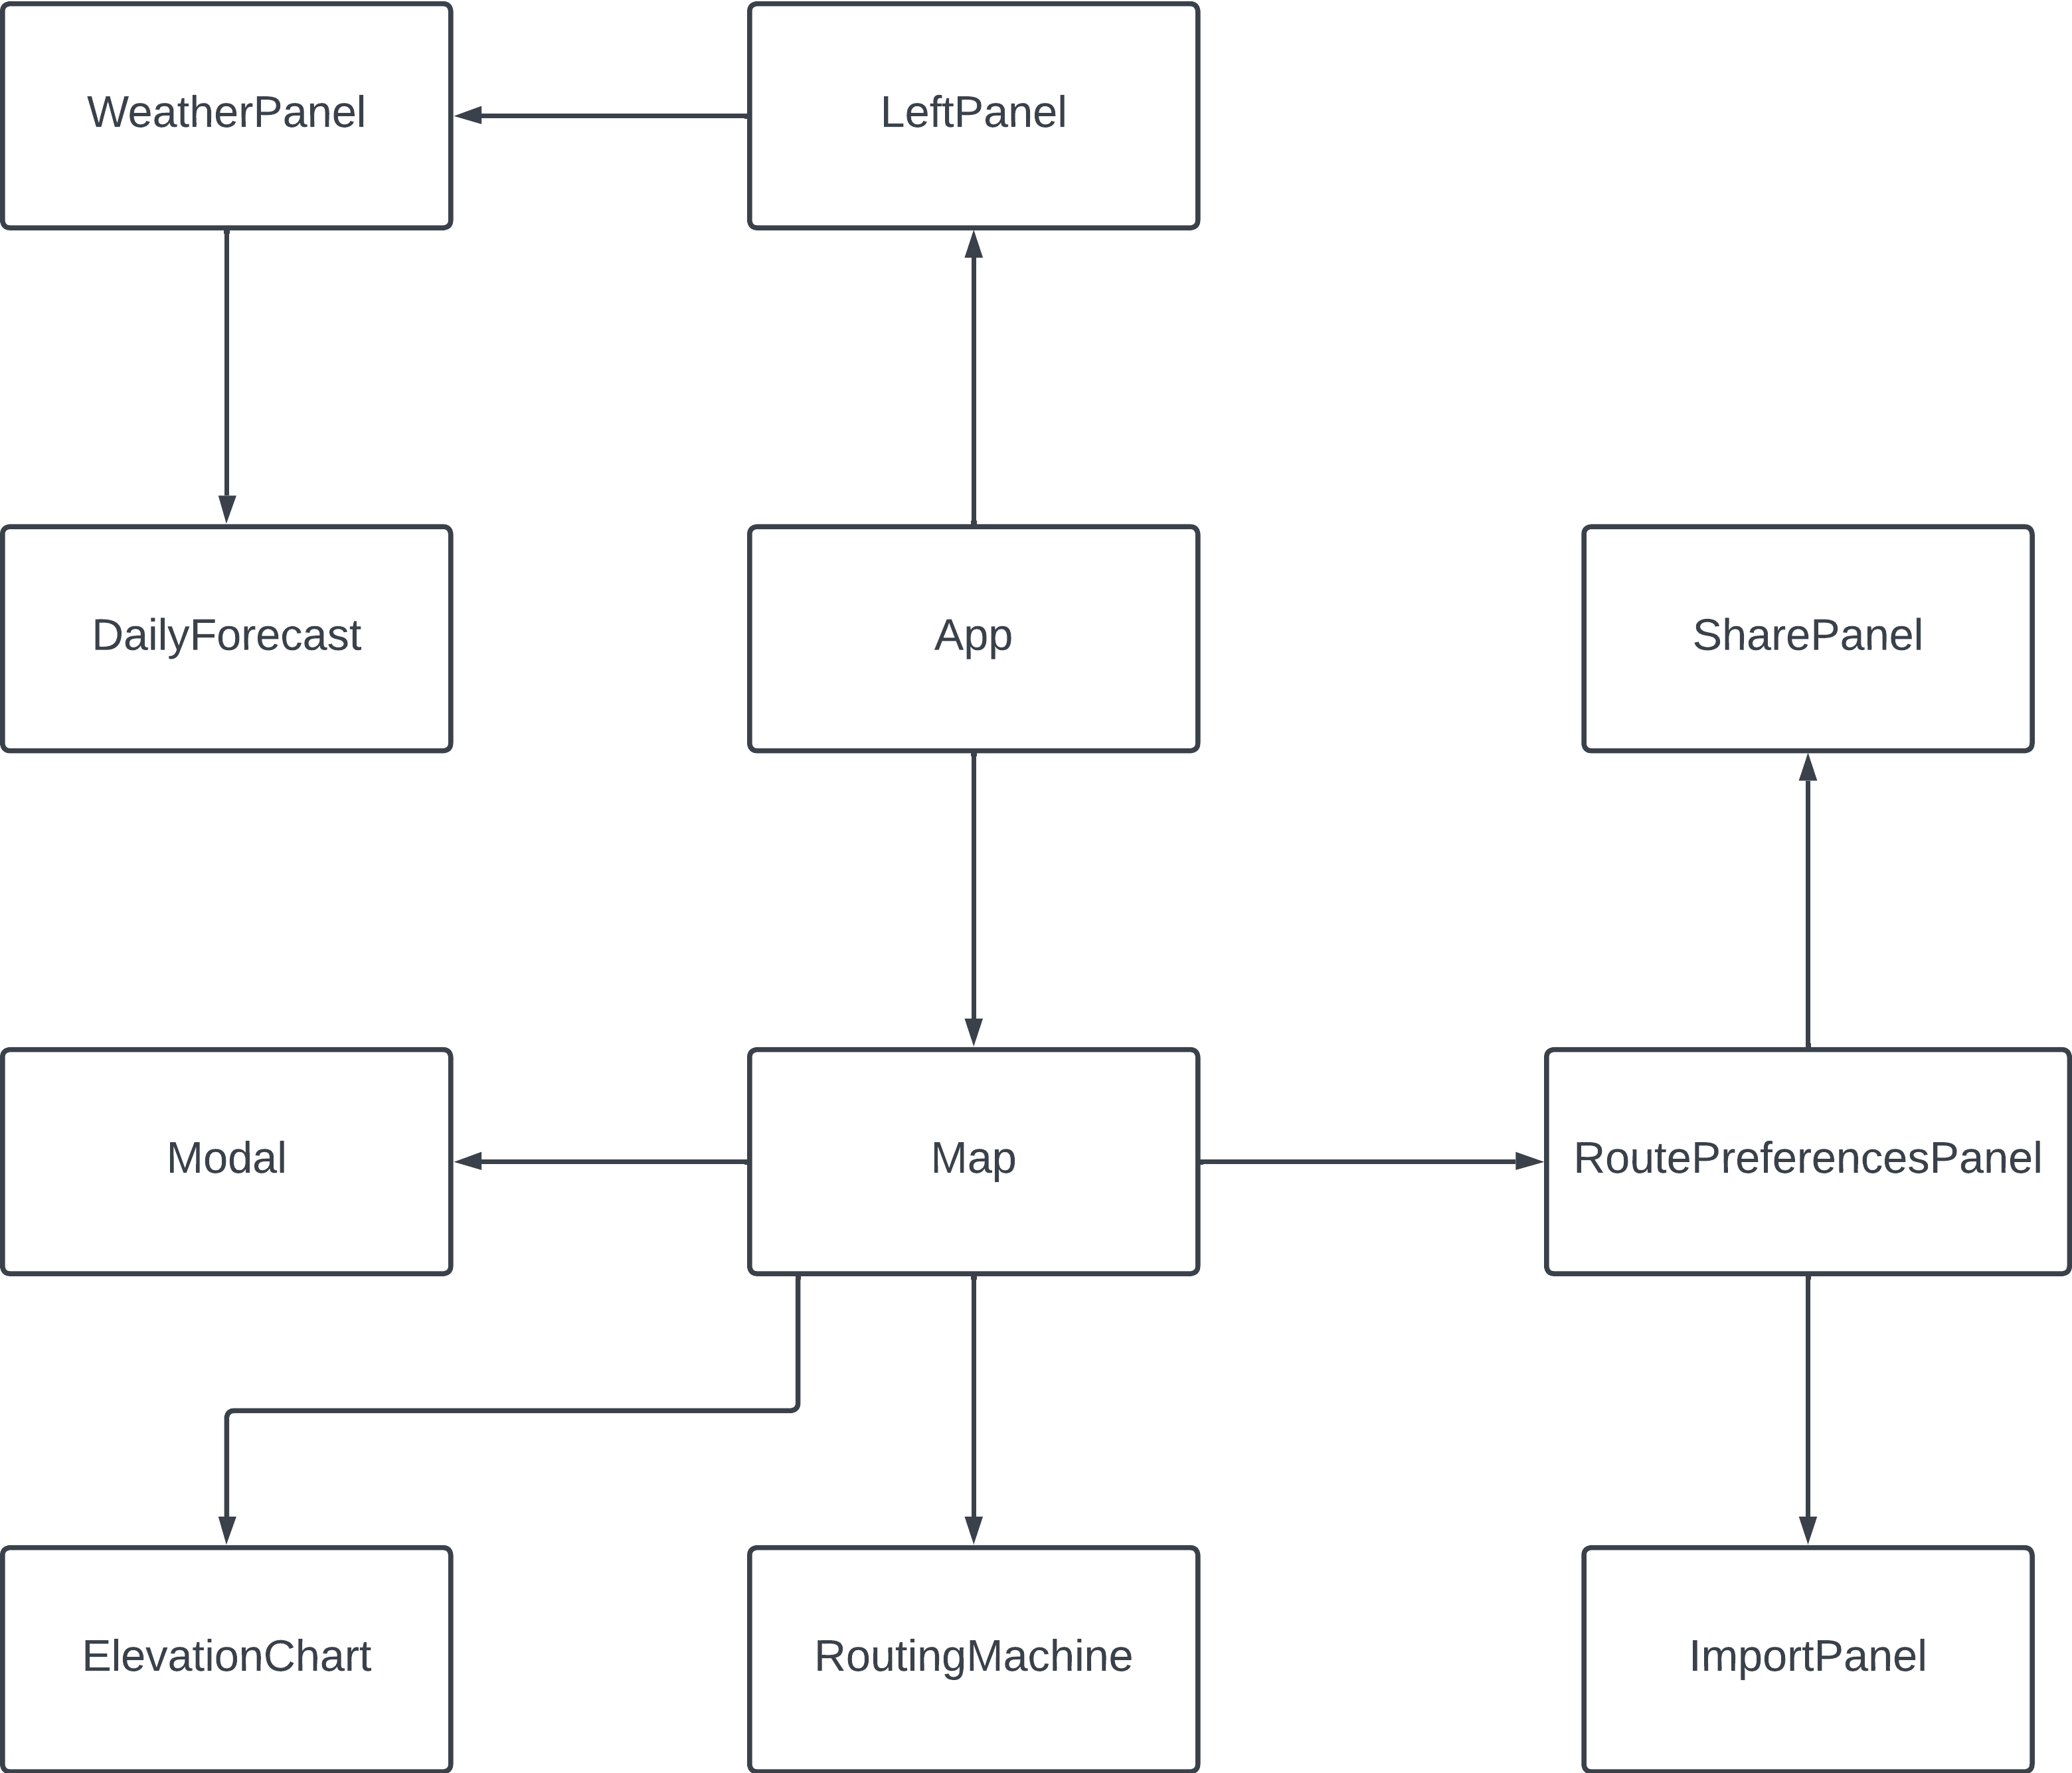
\includegraphics[width=350px]{figures/components.png}
  \caption{Modular Components}
  \label{fig:components}
\end{figure}


\section{Critique of Designs}
\label{design:critique}